% Template for a Computer Science Tripos Part II project dissertation
\documentclass[12pt,a4paper,twoside,openright]{report}
\usepackage[pdfborder={0 0 0}]{hyperref}    % turns references into hyperlinks
\usepackage[margin=25mm]{geometry}  % adjusts page layout
\usepackage{graphicx}  % allows inclusion of PDF, PNG and JPG images
\usepackage{verbatim}
\usepackage{docmute}   % only needed to allow inclusion of proposal.tex

\raggedbottom                           % try to avoid widows and orphans
\sloppy
\clubpenalty1000%
\widowpenalty1000%

\renewcommand{\baselinestretch}{1.1}    % adjust line spacing to make
                                        % more readable

\begin{document}

\bibliographystyle{plain}


%%%%%%%%%%%%%%%%%%%%%%%%%%%%%%%%%%%%%%%%%%%%%%%%%%%%%%%%%%%%%%%%%%%%%%%%
% Title


\pagestyle{empty}

\rightline{\LARGE \textbf{Martin Richards}}

\vspace*{60mm}
\begin{center}
\Huge
\textbf{How to write a dissertation in \LaTeX} \\[5mm]
Computer Science Tripos -- Part II \\[5mm]
St John's College \\[5mm]
\today  % today's date
\end{center}

%%%%%%%%%%%%%%%%%%%%%%%%%%%%%%%%%%%%%%%%%%%%%%%%%%%%%%%%%%%%%%%%%%%%%%%%%%%%%%
% Proforma, table of contents and list of figures

\pagestyle{plain}

\chapter*{Proforma}

{\large
\begin{tabular}{ll}
Name:               & \bf Martin Richards                       \\
College:            & \bf St John's College                     \\
Project Title:      & \bf How to write a dissertation in \LaTeX \\
Examination:        & \bf Computer Science Tripos -- Part II, July 2001  \\
Word Count:         & \bf 1587\footnotemark[1]
                      (well less than the 12000 limit)  \\
Project Originator: & Dr M.~Richards                    \\
Supervisor:         & Dr Markus Kuhn                    \\ 
\end{tabular}
}
\footnotetext[1]{This word count was computed
by \texttt{detex diss.tex | tr -cd '0-9A-Za-z $\tt\backslash$n' | wc -w}
}
\stepcounter{footnote}


\section*{Original Aims of the Project}

To write a demonstration dissertation\footnote{A normal footnote without the
complication of being in a table.} using \LaTeX\ to save
student's time when writing their own dissertations. The dissertation
should illustrate how to use the more common \LaTeX\ constructs. It
should include pictures and diagrams to show how these can be
incorporated into the dissertation.  It should contain the entire
\LaTeX\ source of the dissertation and the makefile.  It should
explain how to construct an MSDOS disk of the dissertation in
Postscript format that can be used by the book shop for printing, and,
finally, it should have the prescribed layout and format of a diploma
dissertation.


\section*{Work Completed}

All that has been completed appears in this dissertation.

\section*{Special Difficulties}

Learning how to incorporate encapulated postscript into a \LaTeX\
document on both Ubuntu Linux and OS X.
 
\newpage
\section*{Declaration}

I, [Name] of [College], being a candidate for Part II of the Computer
Science Tripos [or the Diploma in Computer Science], hereby declare
that this dissertation and the work described in it are my own work,
unaided except as may be specified below, and that the dissertation
does not contain material that has already been used to any substantial
extent for a comparable purpose.

\bigskip
\leftline{Signed [signature]}

\medskip
\leftline{Date [date]}

\tableofcontents

\listoffigures

\newpage
\section*{Acknowledgements}

This document owes much to an earlier version written by Simon Moore
\cite{Moore95}.  His help, encouragement and advice was greatly 
appreciated.

%%%%%%%%%%%%%%%%%%%%%%%%%%%%%%%%%%%%%%%%%%%%%%%%%%%%%%%%%%%%%%%%%%%%%%%
% now for the chapters

\pagestyle{headings}

\chapter{Introduction}

\section{Overview of the files}

This document consists of the following files:

\begin{itemize}
\item \texttt{makefile} --- The makefile for the dissertation and
                         Project Proposal
\item \texttt{diss.tex} --- The dissertation
\item \texttt{proposal.tex}  --- The project proposal 
\item \texttt{figs} -- A directory containing diagrams and pictures
\item \texttt{refs.bib} --- The bibliography database
\end{itemize}

\section{Building the document}

This document was produced using \LaTeXe which is based upon
\LaTeX\cite{Lamport86}.  To build the document you first need to
generate \texttt{diss.aux} which, amongst other things, contains the
references used.  This if done by executing the command:

\texttt{pdflatex diss}

\noindent
Then the bibliography can be generated from \texttt{refs.bib} using:

\texttt{bibtex diss}

\noindent
Finally, to ensure all the page numbering is correct run \texttt{pdflatex}
on \texttt{diss.tex} until the \texttt{.aux} files do not change.  This
usually takes 2 more runs.

\subsection{The makefile}

To simplify the calls to \texttt{pdflatex} and \texttt{bibtex}, 
a makefile has been provided, see Appendix~\ref{makefile}. 
It provides the following facilities:

\begin{description}

\item\texttt{make} \\
 Display help information.

\item\texttt{make proposal.pdf} \\
 Format the proposal document as a PDF.

\item\texttt{make view-proposal} \\
 Run \texttt{make proposal.pdf} and then display it with a Linux PDF viewer
 (preferably ``okular'', if that is not available fall back to ``evince'').

\item\texttt{make diss.pdf} \\
 Format the dissertation document as a PDF.

\item\texttt{make count} \\
Display an estimate of the word count.

\item\texttt{make all} \\
Construct \texttt{proposal.pdf} and \texttt{diss.pdf}.

\item\texttt{make pub} \\ Make \texttt{diss.pdf}
and place it in my \texttt{public\_html} directory.

\item\texttt{make clean} \\ Delete all intermediate files except the
source files and the resulting PDFs. All these deleted files can
be reconstructed by typing \texttt{make all}.

\end{description}


\section{Counting words}

An approximate word count of the body of the dissertation may be
obtained using:

\texttt{wc diss.tex}

\noindent
Alternatively, try something like:

\verb/detex diss.tex | tr -cd '0-9A-Z a-z\n' | wc -w/


\chapter{Preparation}

This chapter is empty!


\chapter{Implementation}

\section{Verbatim text}

Verbatim text can be included using \verb|\begin{verbatim}| and
\verb|\end{verbatim}|. I normally use a slightly smaller font and
often squeeze the lines a little closer together, as in:

{\renewcommand{\baselinestretch}{0.8}\small
\begin{verbatim}
GET "libhdr"
 
GLOBAL { count:200; all  }
 
LET try(ld, row, rd) BE TEST row=all
                        THEN count := count + 1
                        ELSE { LET poss = all & ~(ld | row | rd)
                               UNTIL poss=0 DO
                               { LET p = poss & -poss
                                 poss := poss - p
                                 try(ld+p << 1, row+p, rd+p >> 1)
                               }
                             }
LET start() = VALOF
{ all := 1
  FOR i = 1 TO 12 DO
  { count := 0
    try(0, 0, 0)
    writef("Number of solutions to %i2-queens is %i5*n", i, count)
    all := 2*all + 1
  }
  RESULTIS 0
}
\end{verbatim}
}

\section{Tables}

\begin{samepage}
Here is a simple example\footnote{A footnote} of a table.

\begin{center}
\begin{tabular}{l|c|r}
Left      & Centred & Right \\
Justified &         & Justified \\[3mm]
%\hline\\%[-2mm]
First     & A       & XXX \\
Second    & AA      & XX  \\
Last      & AAA     & X   \\
\end{tabular}
\end{center}

\noindent
There is another example table in the proforma.
\end{samepage}

\section{Simple diagrams}

Simple diagrams can be written directly in \LaTeX.  For example, see
figure~\ref{latexpic1} on page~\pageref{latexpic1} and see
figure~\ref{latexpic2} on page~\pageref{latexpic2}.

\begin{figure}
\setlength{\unitlength}{1mm}
\begin{center}
\begin{picture}(125,100)
\put(0,80){\framebox(50,10){AAA}}
\put(0,60){\framebox(50,10){BBB}}
\put(0,40){\framebox(50,10){CCC}}
\put(0,20){\framebox(50,10){DDD}}
\put(0,00){\framebox(50,10){EEE}}

\put(75,80){\framebox(50,10){XXX}}
\put(75,60){\framebox(50,10){YYY}}
\put(75,40){\framebox(50,10){ZZZ}}

\put(25,80){\vector(0,-1){10}}
\put(25,60){\vector(0,-1){10}}
\put(25,50){\vector(0,1){10}}
\put(25,40){\vector(0,-1){10}}
\put(25,20){\vector(0,-1){10}}

\put(100,80){\vector(0,-1){10}}
\put(100,70){\vector(0,1){10}}
\put(100,60){\vector(0,-1){10}}
\put(100,50){\vector(0,1){10}}

\put(50,65){\vector(1,0){25}}
\put(75,65){\vector(-1,0){25}}
\end{picture}
\end{center}
\caption{A picture composed of boxes and vectors.}
\label{latexpic1}
\end{figure}

\begin{figure}
\setlength{\unitlength}{1mm}
\begin{center}

\begin{picture}(100,70)
\put(47,65){\circle{10}}
\put(45,64){abc}

\put(37,45){\circle{10}}
\put(37,51){\line(1,1){7}}
\put(35,44){def}

\put(57,25){\circle{10}}
\put(57,31){\line(-1,3){9}}
\put(57,31){\line(-3,2){15}}
\put(55,24){ghi}

\put(32,0){\framebox(10,10){A}}
\put(52,0){\framebox(10,10){B}}
\put(37,12){\line(0,1){26}}
\put(37,12){\line(2,1){15}}
\put(57,12){\line(0,2){6}}
\end{picture}

\end{center}
\caption{A diagram composed of circles, lines and boxes.}
\label{latexpic2}
\end{figure}



\section{Adding more complicated graphics}

The use of \LaTeX\ format can be tedious and it is often better to use
encapsulated postscript (EPS) or PDF to represent complicated graphics.
Figure~\ref{epsfig} and~\ref{xfig} on page \pageref{xfig} are
examples. The second figure was drawn using \texttt{xfig} and exported in
{\tt.eps} format. This is my recommended way of drawing all diagrams.


\begin{figure}[tbh]
\centerline{
\includegraphics{figs/cuarms.pdf}}
\caption{Example figure using encapsulated postscript}
\label{epsfig}
\end{figure}

\begin{figure}[tbh]
\vspace{4in}
\caption{Example figure where a picture can be pasted in}
\label{pastedfig}
\end{figure}


\begin{figure}[tbh]
\centerline{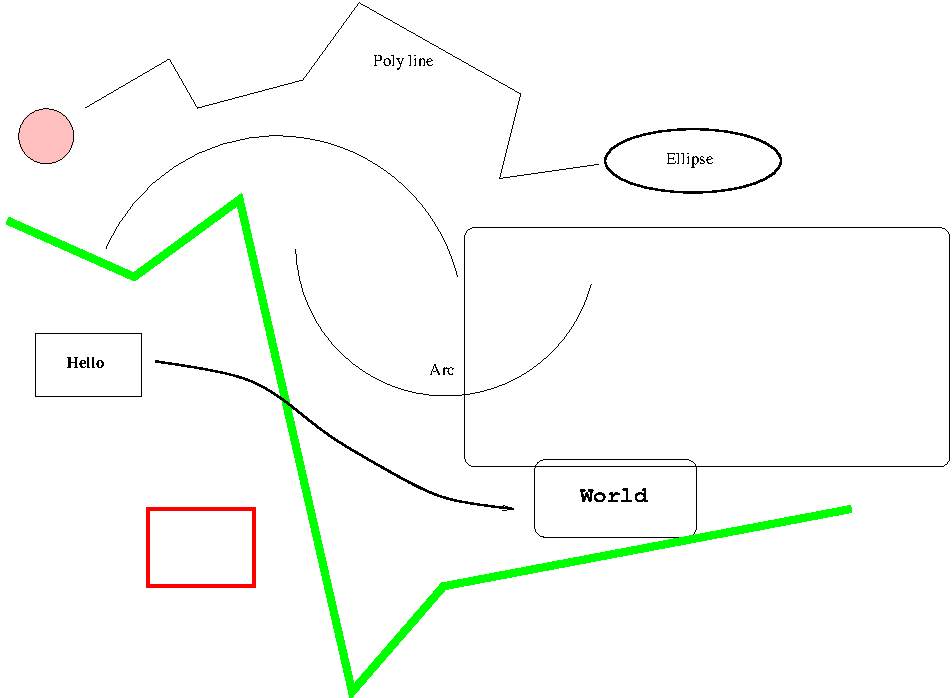
\includegraphics{figs/diagram.pdf}}
\caption{Example diagram drawn using \texttt{xfig}}
\label{xfig}
\end{figure}


\chapter{Evaluation}

\section{Printing and binding}

Use a ``duplex'' laser printer that can print on both sides to print
two copies of your dissertation. Then bind them, for example using the
comb binder in the Computer Laboratory Library.

\section{Further information}

See the Unix Tools notes at

\url{http://www.cl.cam.ac.uk/teaching/current-1/UnixTools/materials.html}


\chapter{Conclusion}

I hope that this rough guide to writing a dissertation is \LaTeX\ has
been helpful and saved you time.


%%%%%%%%%%%%%%%%%%%%%%%%%%%%%%%%%%%%%%%%%%%%%%%%%%%%%%%%%%%%%%%%%%%%%
% the bibliography
\addcontentsline{toc}{chapter}{Bibliography}
\bibliography{refs}

%%%%%%%%%%%%%%%%%%%%%%%%%%%%%%%%%%%%%%%%%%%%%%%%%%%%%%%%%%%%%%%%%%%%%
% the appendices
\appendix

\chapter{Latex source}

\section{diss.tex}
{\scriptsize\verbatiminput{diss.tex}}

\section{proposal.tex}
{\scriptsize\verbatiminput{proposal.tex}}

\chapter{Makefile}

\section{makefile}\label{makefile}
{\scriptsize\verbatiminput{makefile.txt}}

\section{refs.bib}
{\scriptsize\verbatiminput{refs.bib}}


\chapter{Project Proposal}

% arara: lualatex
% Note: this file can be compiled on its own, but is also included by
% diss.tex (using the docmute.sty package to ignore the preamble)
\documentclass[12pt,a4paper,twoside]{article}
\usepackage[pdfborder={0 0 0}]{hyperref}
\usepackage[margin=25mm]{geometry}
\usepackage{graphicx}
\usepackage{parskip}

\begin{document}

\begin{center}
    \Large
    Computer Science Tripos -- Part II -- Project Proposal\\[4mm]
    \LARGE
    A strongly consistent index for email using git and MirageOS.

    \large
    O.~Hope, Jesus College

    Originator: Dr A.~Madhavapeddy

    18th October 2018
\end{center}

\vspace{5mm}

\textbf{Project Supervisor:} Mr D.~Allsopp

\textbf{Director of Studies:} Prof C.~Mascolo

\textbf{Project Overseers:} Prof G.~Winskel \& Dr R.~Mortier

% Main document

\section*{Introduction}

Maildir is a widely used format for storing emails. Its main benefit is that it uses the filesystem in such a way that client programs do not have to handle locking themselves. The downside of this is that it makes it hard to create a consistent index as we cannot guarantee that the filesystem is in a consistent state when we try to update it. If we did have a consistent index, it would allow for safer concurrent support and the implementation of new features.

MirageOS is a library operating system for building unikernels written in OCaml. This means that it provides OCaml libraries which can be combined and compiled down into high-performance, lightweight kernels. These can then run directly on a hypervisor and only contain the code required to provide the functionality needed. However, the libraries themselves can also be used outside of unikernels to provide functionality to applications on more standard systems. This will be the use case in this project, using the MirageOS libraries to create a standalone application to run on unix-like systems.

The aim therefore is to solve the consistency problem. This can be done by using git, the version control system, to build an overlay on top of maildir in the filesystem. Then multiple filesystem operations can be bundled into commits. These can be used to track of all changes made to the maildir. As these changes are being recorded by a version control system, we can be sure that any index built on top will be strongly consistent. As git also provides branching, we can extend this model to add new features described in the possible extensions section.

We can implement this git overlay using libraries provided by MirageOS which provide git functionality, maildir operations, and even email parsing. With the overlay, and therefore consistent index implemented, we will then be able to make many more guarantees about the state of the maildir at any time. This will also allow for dealing with conflicting operations in an easier and more reliable manner. Furthermore, the overlay will also provide the possibility of easily implementing novel features such as roll-back and separate branches for different use cases.

\section*{Starting point}

I have used git for version control of software projects in the past, so I have a basic understanding of some of its more commonly used features when using it as a tool. However, I have little knowledge of its more low level actions which will be needed when managing filesystem operations.

MirageOS provides some libraries meaning that I will not have to implement some features from scratch. These include ocaml-git to manage git operations, a library for actioning maildir operations, and one which supports email file parsing.

I have previous experience in Standard ML from the Foundations of Computer Science course in Part IA, but most of the differences and extra features in OCaml will be new to me.

\section*{Resources required}

For this project I will use my own Apple Macbook Pro (2018) running macOS.
I will backup all of my work on a Github repository, and will make weekly backups of my entire computer to an external hard drive. Should my laptop suddenly fail, I have a spare and the option to use the MCS computers in the Computer Laboratory. Alongside my computer, I will take a snapshot of my personal Cambridge email account at the start of the project for testing purposes all other tests will be performed with generated mailboxes. I will require no other special resources.

\section*{Work to be done}

The project breaks down into the following sub-projects:

\begin{enumerate}

    \item \textbf{Designing overlay functionality:} Working out exactly what git features will be needed for the required overlay functionality, how they fit together, and designing a strategy to implement this.

    \item \textbf{Prototyping the overlay:} Building a version of the overlay to work using standard command line tools (including git) and non-mirage scripts.

    \item \textbf{Adding index functionality:} Using the overlay to actually implement the prototype of the consistent indexing.

    \item \textbf{Adapting the overlay to MirageOS:} Implementing the overlay with MirageOS libraries and OCaml using the knowledge gained whilst prototyping, using pre-existing libraries to manage the git and filesystem operations.

    \item \textbf{Testing and Evaluation:} Checking that all maildir operations continue to work as expected, testing the index for strong consistency. Testing resolution of conflicts from concurrent operations. Quantifying the slow-down relative to maildir with no consistent index over operations such as insertion and deletion of emails in different quantities and concurrent actions from different processes.

\end{enumerate}

\section*{Success criteria}

The success of the project will be evaluated against:

\begin{enumerate}

    \item Implementation of a working git overlay on top of the filesystem in MirageOS.

    \item A strongly consistent maildir index using the git overlay which allows all standard maildir operations.

\end{enumerate}

\section*{Possible extensions}

If I finish both my implementation and evaluation of the project early, then it could be extended by implementing:

\begin{itemize}

    \item Rollback support in case of user errors such as accidental deletion.

    \item Branch support to process emails for different platforms. For example a branch for mobile clients which has all images removed from the emails to reduce mobile data usage.

    \item Intelligently handling conflicts such as replying to the same message twice from different clients.

\end{itemize}

\section*{Timetable}

Planned starting date is 22/10/2018.

\begin{enumerate}

    \item \textbf{Michaelmas weeks 2--4 (22nd October--31st October):} Read through the full git documentation of all the standard features, research the maildir format, evaluate different indexing techniques, start learning OCaml, and take a snapshot of my Cambridge email account.

        \emph{Milestone: Have decided on a high level implementation strategy}

    \item \textbf{Michaelmas weeks 5--6 (1st November--14th November):} Write the prototype overlay using git on a standard OS (macOS) and continue learning OCaml.

    \item \textbf{Michaelmas weeks 7--8 (15th November--28th November):} Add the indexing functionality, test under all the necessary operations, read the MirageOS documentation relating to the filesystem, git operations, and any other libraries that will be needed.

        \emph{Milestone: Prototype implementation complete}

    \item \textbf{Michaelmas vacation weeks 1--2 (29th November--12th December):} Start implementation of the overlay in OCaml.

    \item \textbf{Michaelmas vacation weeks 6--7 (3rd January--16th January):} Continue implementation of overlay in OCaml, and test index is consistent for all operations.

        \emph{Milestone: OCaml application complete}

    \item \textbf{Lent weeks 1--2 (17th January--30th January):} Write progress report. Start to set up further tests for the application and begin evaluating its features.

    \item \textbf{Lent weeks 3--4 (31st January--5th February):} Set up and perform tests to evaluate the performance of the overlay under different operations and maildir conditions.

        \emph{Milestone: Testing of all basic features complete}

    \item \textbf{Lent weeks 5--6 (14th February--27th February):} Implement possible extensions if all previous milestones met and begin writing main dissertation chapters.

    \item \textbf{Lent weeks 7--8 (28th February--13th March):} Complete dissertation first draft and complete extensions.

        \emph{Milestone: Dissertation draft complete}

    \item \textbf{Easter vacation (20th March--24th April):} Start revising dissertation using feedback given, and complete any remaining evaluations.

    \item \textbf{Easter term weeks 1--2 (25th April--8th May):} Complete dissertation final draft.

        \emph{Milestone: Dissertation complete}

    \item \textbf{Easter term week 3 (9th May--15th May):} Any remaining proofreading, and an early submission to concentrate on exam revision.

        \emph{Milestone: Dissertation submitted}

\end{enumerate}

\end{document}


\end{document}
